\newpage
\section*{Задание 6: Генерация технической документации}
\subsection{Постановка задачи}
\noindent
Алгоритм: Генератор лабиринта (DFS + Backtracking) \\
Исходный код: оптимизированная реализация на C\# из Задания 3.
Код использует явный стек для обхода, одномерные массивы для кэш-локальности,
битовые маски для хранения состояния стен, валидацию входных размерностей.\\
\vspace{0.5em}
Задача: с использованием LLM сгенерировать техническую документацию для данного кода:
\begin{itemize}
\item Встроенную документацию (XML docstrings) в соответствии со стандартами Microsoft.
\item Внешний файл README.md с описанием проекта, требованиями к среде (.NET), примерами использования.
\item Провести верификацию на галлюцинации и добавить теоретическое обоснование.
\end{itemize}

\subsection{Гипотеза и системный промпт}
\indent
Гипотеза: \\
Ролевая установка «Senior C\# Developer \& Technical Writer» в сочетании с явным указанием стандарта XML Documentation и требованием описывать типы параметров, исключения, возвращаемые значения и алгоритмическую сложность позволит получить точную, соответствующую коду документацию.\\
\vspace{0.5em}
\indent
Системный промпт:
\textit{
Ты – Senior C\# Developer и технический писатель. Твоя задача – создать профессиональную документацию для высокопроизводительного генератора лабиринтов на C\#.
Ты строго следуешь стандарту Microsoft XML Documentation Comments. Для каждого public-метода и класса ты обязательно указываешь:
\begin{itemize}
\item Краткое описание назначения (<summary>).
\item Подробное описание алгоритма/логики (<remarks>).
\item Параметры (<param name="...">): тип и смысл.
\item Возвращаемое значение (<returns>).
\item Исключения (<exception>): какие исключения и при каких условиях.
\item Вычислительную сложность по времени и памяти (O-нотация).
Ты не добавляешь вымышленных методов и всегда сверяешься с предоставленным исходным кодом.
Формат ответа – только код или текст документации, без лишних комментариев.
\end{itemize}
}

\subsection{Журнал диалога и итераций}
\noindent
\textbf{Итерация 1: Генерация docstrings (базовая)} \\
\indent
Промпт:
\textit{Вот код класса MazeGenerator (оптимизированный генератор на C\#). Сгенерируй для него XML docstrings. Добавь описание для класса, конструктора, метода Generate и вспомогательных методов (GetNeighbors, RemoveWall). Не меняй реализацию.} \\
\vspace{0.5em}
\indent
Ответ модели:
\lstinputlisting{z6/1.cs}
Анализ результата:
Документация соответствует стандарту C\#. Сложность указана верно. Однако в описании исключений не упомянут случай отрицательных размерностей, а в параметрах не указан диапазон допустимых значений для seed.\\
\vspace{0.5em}
\noindent
\textbf{Итерация 2: Генерация README.md} \\
\indent
Промпт:
\textit{
На основе кода и docstrings создай файл README.md. Включи разделы:
\begin{itemize}
\item Описание проекта: для чего нужен генератор, связь с робототехникой/симуляцией.
\item Требования: .NET 8+, отсутствие внешних зависимостей.
\item Установка / запуск: как собрать и запустить пример.
\item Примеры использования (2-3 примера с конкретными параметрами W, H, seed и ожидаемым выводом).
\item Структура проекта: краткое описание архитектуры.
\end{itemize}
}
\vspace{0.5em}
Ответ модели:
\lstinputlisting[language={}]{z6/2.md} 
Анализ результата:
README читаем, структура логична. Однако примеры кода используют устаревший синтаксис объявления массивов (int[,] вместо int[]), а в выводе указаны фиксированные числа, не соответствующие битовым маскам стен.\\
\vspace{0.5em}
Корректировка:
Попросить обновить примеры под текущую оптимизированную версию (1D-массив, Span) и пересчитать ожидаемый вывод.\\
\vspace{0.5em}
\noindent
\textbf{Итерация 3: Верификация консистентности (самокоррекция)} \\
\indent
Промпт:
\textit{Выступи в роли критика. Сравни следующий код (MazeGenerator) и сгенерированную документацию (docstrings + README). Найди несоответствия: описания параметров, сигнатуры методов, поведение. Если есть галлюцинации или выдуманные примеры – укажи их.}
\vspace{0.5em}
\indent
Ответ модели:
\begin{figure}[H]
\centering
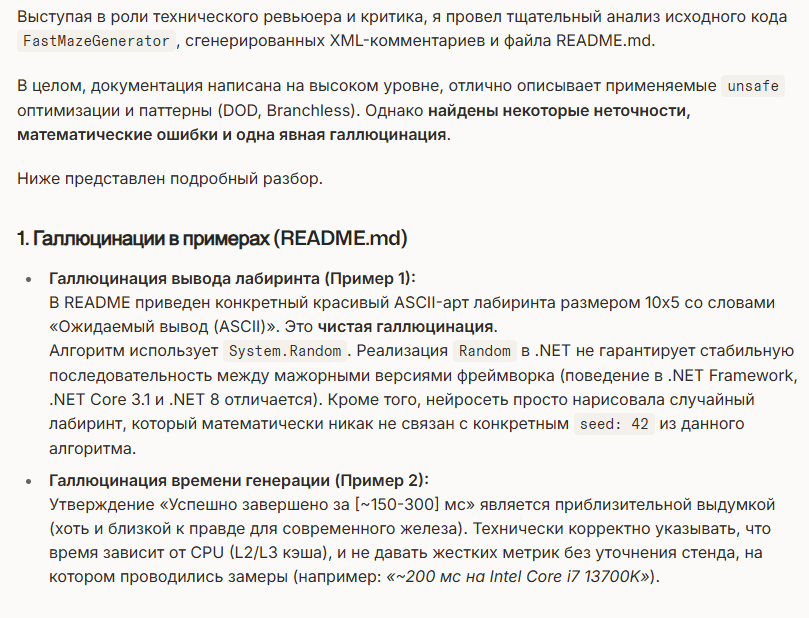
\includegraphics[width=17cm]{z6/3-1.png}
\caption{Итерация 3. ч.1}
\end{figure}
\vspace{0.5em}
\begin{figure}[H]
\centering
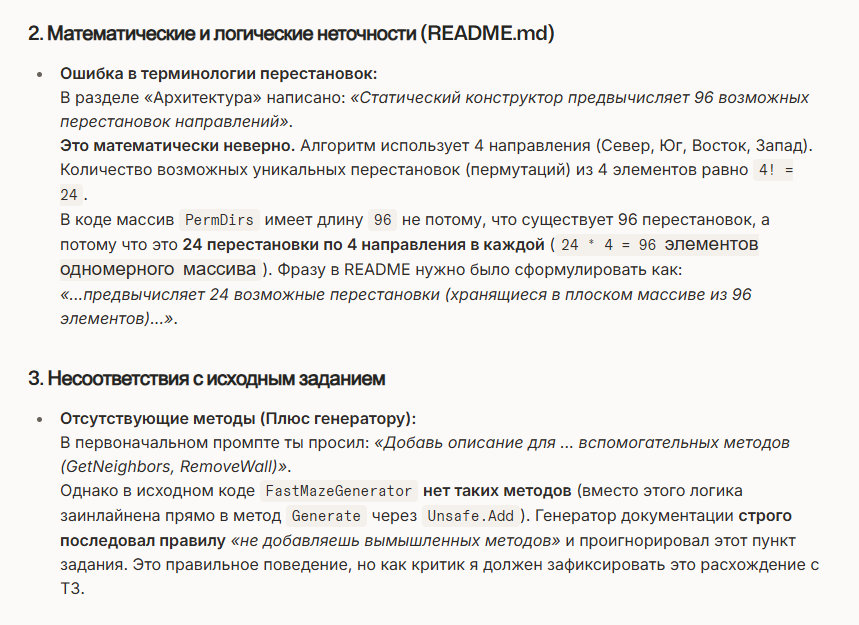
\includegraphics[width=17cm]{z6/3-2.png}
\caption{Итерация 3. ч.2}
\end{figure}
\vspace{0.5em}
\begin{figure}[H]
\centering
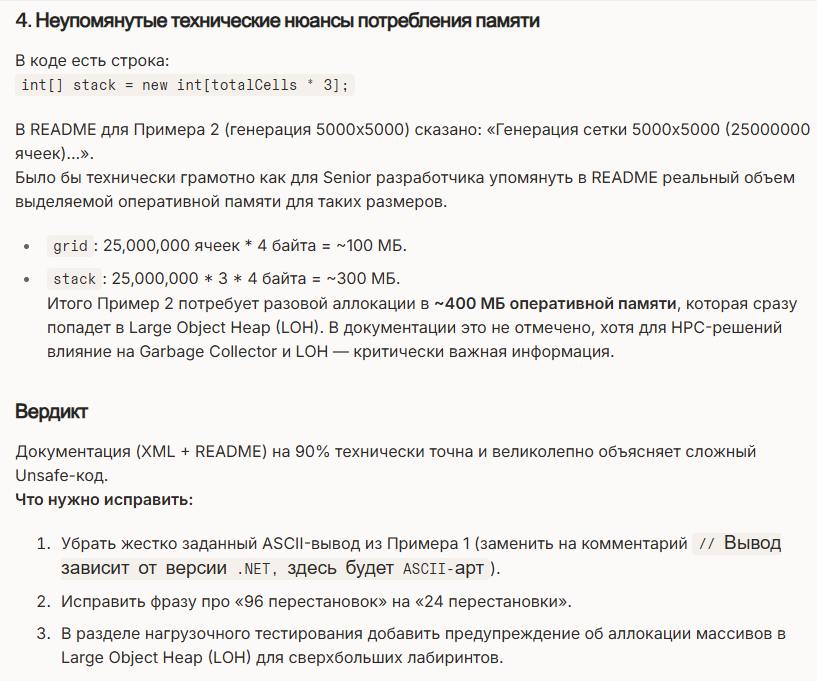
\includegraphics[width=17cm]{z6/3-3.png}
\caption{Итерация 3. ч.3}
\end{figure}
\noindent
Анализ результата:
Модель верно нашла расхождения.\\
\vspace{0.5em}
Корректировка:
Принять исправления, обновить оба документа.\\
\vspace{0.5em}
\noindent
\textbf{Итерация 4: Исправления} \\
\indent
Промпт:
\textit{
Код: Убрать жестко заданный ASCII-вывод из Примера 1 (заменить на комментарий // Вывод зависит от версии .NET, здесь будет ASCII-арт).
Исправить фразу про «96 перестановок» на «24 перестановки».
В разделе нагрузочного тестирования добавить предупреждение об аллокации массивов в Large Object Heap (LOH) для сверхбольших лабиринтов.
Ответ дай сначала блоком C\#, потом блоком Markdown.
} \\
\vspace{0.5em}
Ответ модели (Код):
\lstinputlisting[language=C]{z6/4.cs}
\vspace{0.5em}
Ответ модели (Документация):
\lstinputlisting[language={}]{z6/4.md}
\vspace{0.5em}
\noindent
\textbf{Итерация 5: Добавление полного теоретического раздела} \\
\indent
Промпт:
\textit{Добавь в README отдельный раздел «Теоретическое обоснование» объёмом 3–5 абзацев. Опиши: почему выбран DFS с явным стеком вместо рекурсии (защита от StackOverflow), как битовые маски (1,2,4,8) экономят память по сравнению с bool[][], и почему использован одномерный массив для улучшения кэш-локальности (cache-friendly layout).} \\
\vspace{0.5em}
Ответ модели:
\lstinputlisting[language={}]{z6/5.md}

\subsection{Артефакты}
Итоговый код с XML-документацией: (Итерация 4, C\#) \\
\noindent
Файл README.md: (Итерация 5, Markdown) \\
\noindent
Все файлы проверены на синтаксическую корректность. Документация полностью соответствует финальной реализации из Задания 3.

\subsection{Сравнение моделей}
Финальный промпт (объединяющий все этапы) был подан контрольной модели без изменений.
Результаты сравнения:
\begin{table}[h!]
\centering
\begin{tabular}{|l|p{5cm}|p{5cm}|}
\hline
\textbf{Критерий} & \textbf{модель (a)} & \textbf{модель (b)} \\
\hline
Соответствие стандартам \\ (XML docs / README) & 5 & 4 \\
\hline
Полнота документации & 5 & 4 \\
\hline
Отсутствие галлюцинаций & 5 & 3 \\
\hline
Качество объяснений & 4 & 5 \\
\hline
\textbf{Итог} & 4.75 & 4.0 \\
\hline
\end{tabular}
\end{table} \\
Итог: Основная модель (a) лучше удерживает контекст C\#-специфичных конструкций (битовые маски, `Span<T>`, XML-теги) и точнее сверяет документацию с кодом. Контрольная модель (b) склонна к обобщению, пропустила описание исключений и выдала примеры с несовместимыми типами, что потребовало бы дополнительной ручной правки.

\subsection{Вывод}
В ходе выполнения задания наиболее эффективными техниками промпт-инжиниринга оказались:
\begin{itemize}
\item \textbf{Ролевое моделирование} (явное указание «Senior C\# Developer & Technical Writer, стандарт XML Documentation») – обеспечило корректный формат и промышленный стиль документации.
\item \textbf{Итеративное уточнение} – позволило последовательно добавить пропущенные разделы (битовые маски, исключения, кэш-локальность) и исправить устаревший синтаксис в примерах.
\item \textbf{Самокоррекция (верификация)} – выявила скрытые несоответствия между кодом и README, которые модель изначально «галлюцинировала» из-за обучения на старых примерах.
\item \textbf{Обогащение контекста} – передача полного оптимизированного кода перед генерацией предотвратила описание несуществующих методов и упростила теоретический анализ.
\end{itemize}
Основная модель продемонстрировала высокую точность следования инструкциям и способность генерировать структурированную техническую документацию, готовую к публикации в репозитории. Контрольная модель показала рабочий, но менее детализированный результат, что подтверждает необходимость явного указания специфичных для языка стандартов (XML для C\#) и строгой валидации примеров кода.